\documentclass[conference]{IEEEtran}
\IEEEoverridecommandlockouts

\usepackage[utf8]{inputenc}
\usepackage[T1]{fontenc}
\usepackage[spanish,es-nodecimaldot]{babel}
\usepackage{amsmath,amssymb,amsfonts,bm}
\usepackage{graphicx}
\usepackage{booktabs}
\usepackage{array}
\usepackage{cite}
\usepackage{textcomp}
\usepackage[hidelinks]{hyperref}

\graphicspath{{figures/}}

% ---------- Macros ----------
\newcommand{\bp}{\bm{p}}
\newcommand{\bv}{\bm{v}}
\newcommand{\bx}{\bm{x}}
\newcommand{\bu}{\bm{u}}
\newcommand{\bz}{\bm{z}}
\newcommand{\bef}{\bm{f}}
\newcommand{\bd}{\bm{d}}
\newcommand{\bomega}{\bm{\omega}}
\newcommand{\btau}{\bm{\tau}}
\newcommand{\bR}{\mathbf{R}}
\newcommand{\RR}{\mathbb{R}}
\newcommand{\tr}{^{\top}}
\newcommand{\mg}{mg}

\def\BibTeX{{\rm B\kern-.05em{\sc i\kern-.025em b}\kern-.08em
    T\kern-.1667em\lower.7ex\hbox{E}\kern-.125em X}}

% Los captions de tablas dicen "Tabla" (babel-spanish usa "Cuadro" por defecto)
\addto\captionsspanish{\renewcommand{\tablename}{Tabla}}

\begin{document}
\title{Control de Actitud y Altura de un Cuadricóptero F450 con ESP32-S3:\\
Identificación de Parámetros, Implementación y Ensayos de Vuelo\\
{\large Robótica Avanzada -- Proyecto del Curso}}

\author{\IEEEauthorblockN{Luis Eduardo Kamt Chang}
\IEEEauthorblockA{\textit{Ingeniería Mecatrónica}\\
\textit{Universidad de Ingeniería y Tecnología}\\
\textit{(UTEC)}\\
Lima, Perú}
\and
\IEEEauthorblockN{Ilianov Nikolay Ore Cruzatt}
\IEEEauthorblockA{\textit{Ingeniería Mecatrónica}\\
\textit{Universidad de Ingeniería y Tecnología}\\
\textit{(UTEC)}\\
Lima, Perú}
\and
\IEEEauthorblockN{Kenyi Stiwar Reyes de Lama}
\IEEEauthorblockA{\textit{Ingeniería Mecatrónica}\\
\textit{Universidad de Ingeniería y Tecnología}\\
\textit{(UTEC)}\\
Lima, Perú}
}

\maketitle

\begin{abstract}
Se documenta el diseño, la implementación y los ensayos de vuelo de un controlador de actitud y altura para un cuadricóptero F450 (1.0022\,kg) gobernado por un ESP32-S3. El controlador sigue la formulación del curso: linealización por realimentación en cascada (ángulo $\to$ velocidad angular $\to$ torque), control de altura con cancelación de gravedad y mezclador por inversión de la matriz de rotores, y se extiende con un integrador, un super-twisting opcional y una identificación recursiva de la autoridad de control. Los parámetros del modelo se obtuvieron experimentalmente: inercias con péndulo bifilar ($I_x=9.71$, $I_y=10.56$, $I_z=20.08\times10^{-3}$\,kg\,m$^2$), el coeficiente de empuje con un banco de motor y el de par a partir de la relación empuje/par de la hélice. Se analizan dos vuelos de la versión V\_11 y se los compara con la V\_10. En el vuelo B el dron despegó y se sostuvo en el aire con $|\phi|<10^{\circ}$ el 78\,\% del tiempo y un pico de $57^{\circ}$ recuperado sin desarme; el estimador de altura mejoró frente a V\_10 (desviación respecto del ultrasonido $0.12$\,m frente a $0.26$--$1.39$\,m), aunque diverge junto al suelo cuando se queda sin medida válida. Se discuten las limitaciones: margen de empuje reducido (relación empuje/peso 1.43), discrepancia entre la curva de empuje de banco y el vuelo, y ausencia de medición de batería y de posición lateral.
\end{abstract}

\begin{IEEEkeywords}
cuadricóptero, linealización por realimentación, control en cascada, identificación de parámetros, filtro de Kalman, super-twisting, ESP32-S3.
\end{IEEEkeywords}

\section{Introducción}
\label{sec:intro}

Un cuadricóptero es un robot aéreo \emph{subactuado}: cuatro entradas (empuje total y tres torques) gobiernan seis grados de libertad, por lo que solo se pueden controlar cuatro salidas independientes. Las notas del curso resuelven este problema separando el movimiento en una dinámica de traslación, cuya entrada es el empuje $u_1$ proyectado por la actitud, y una dinámica de rotación, de la que se encarga un lazo interno rápido; ambas se linealizan por realimentación y se cierran en cascada~\cite{notas1}. La misma formulación advierte que la cancelación exacta depende de un modelo preciso y que las incertidumbres de $m$, $I$ o $k_f$, la saturación de los actuadores y las perturbaciones externas degradan el desempeño, lo que motiva el control adaptativo y robusto del segundo bloque del curso~\cite{notas2}.

Este informe presenta la implementación de esa teoría en un dron real: un marco F450 con cuatro motores A2212 de 1000\,KV, controlado por un ESP32-S3 con IMU MPU-6500, un sensor de distancia láser VL53L0X y un ultrasonido HC-SR04. El firmware evaluado es la versión V\_11 del proyecto. El objetivo es \emph{estabilizar la actitud (roll, pitch, yaw) y mantener la altura} usando un modelo cuyos parámetros se identificaron experimentalmente y evaluar el resultado con las cajas negras de vuelo. No se controla la posición lateral $(x,y)$, porque el dron no dispone de ningún sensor que la mida.

Las contribuciones son: (i) la identificación de masa, inercias y coeficientes del rotor (Sección~\ref{sec:ident}); (ii) un firmware de 250\,Hz que implementa la cascada del curso, un mezclador con prioridad de ejes y un estimador de altura por Kalman, con extensiones robusta y adaptativa (Sección~\ref{sec:control}); y (iii) el análisis cuantitativo de dos vuelos V\_11 y su comparación con V\_10, incluyendo los fallos observados (Sección~\ref{sec:res}). La Sección~\ref{sec:conc} resume las conclusiones.

\section{Metodología}
\label{sec:met}

\subsection{Plataforma experimental}
La Tabla~\ref{tab:hw} resume el hardware. Se adopta la convención de las notas: sistema del cuerpo $\{B\}$ con $x$ hacia adelante, $y$ hacia la derecha y $z$ hacia abajo, ángulos de Euler $ZYX$ y rotores numerados 1 a 4 (adelante-izquierda, adelante-derecha, atrás-derecha, atrás-izquierda) en $\bm r_1=(l,-l,0)$, $\bm r_2=(l,l,0)$, $\bm r_3=(-l,l,0)$, $\bm r_4=(-l,-l,0)$. El dron no tiene medición de tensión de batería ni de posición lateral; esto limita el análisis (Sección~\ref{sec:disc}).

\begin{table}[t]
\caption{Componentes de la plataforma.}
\label{tab:hw}
\centering\small
\begin{tabular}{@{}lp{5.7cm}@{}}
\toprule
Elemento & Descripción \\
\midrule
Marco y propulsión & F450; 4 $\times$ A2212 1000\,KV; hélice APC 10$\times$4.5\,MR \\
Actuación & 4 ESC 30\,A, PWM a 50\,Hz, recorrido 1040--1800\,\textmu{}s \\
Controlador & ESP32-S3 (núcleo 1: control a 250\,Hz; núcleo 0: sensores y web) \\
Actitud & MPU-6500 (I$^2$C), filtro de Mahony \\
Altura & VL53L0X (ToF, útil $<$25\,cm), HC-SR04 (útil 8\,cm--3.5\,m) \\
Enlace & Punto de acceso WiFi y página de control, caja negra a 50\,Hz \\
\bottomrule
\end{tabular}
\end{table}

\subsection{Modelo dinámico}
Se usa el modelo de las notas~\cite{notas1}. Con $\bm\eta=(\phi,\theta,\psi)$ y $\bm\omega=(p,q,r)$ en $\{B\}$, la cinemática de Euler es
\begin{align}
\dot\phi&=p+q\sin\phi\tan\theta+r\cos\phi\tan\theta,\nonumber\\
\dot\theta&=q\cos\phi-r\sin\phi,\label{eq:euler}\\
\dot\psi&=(q\sin\phi+r\cos\phi)/\cos\theta,\nonumber
\end{align}
la traslación, con $u_1=-f_t/m$, es $\ddot x=r_{13}u_1$, $\ddot y=r_{23}u_1$, $\ddot z=g+r_{33}u_1$ con $r_{33}=\cos\theta\cos\phi$, y la rotación es $I\dot{\bm\omega}+\bm\omega\times(I\bm\omega)=\btau$ con $I=\mathrm{diag}(I_x,I_y,I_z)$. Cada rotor produce $f_i=k_f\omega_i^2$ y $\tau_i=k_m\omega_i^2$, de modo que
\begin{equation}
\begin{bmatrix}f_t\\ \tau_x\\ \tau_y\\ \tau_z\end{bmatrix}=
\begin{bmatrix}
k_f&k_f&k_f&k_f\\
k_fl&-k_fl&-k_fl&k_fl\\
k_fl&k_fl&-k_fl&-k_fl\\
k_m&-k_m&k_m&-k_m
\end{bmatrix}
\begin{bmatrix}\omega_1^2\\ \omega_2^2\\ \omega_3^2\\ \omega_4^2\end{bmatrix}.
\label{eq:mezcla}
\end{equation}
Con $\omega_{\min}=0.15\,\omega_{\max}$ y $\omega_{\max}=1046$\,rad/s (estimada a partir de $KV\cdot V_{bat}\cdot\eta$, único parámetro del mapeo que no se midió), el conjunto factible es el politopo $\omega_{\min}^2\le\omega_i^2\le\omega_{\max}^2$.

\subsection{Identificación de parámetros}
\label{sec:ident}
Los parámetros se obtuvieron con tres ensayos (hoja de cálculo del proyecto).

\textbf{Masa y brazo.} La masa en vuelo es $m=1.0022$\,kg. El brazo efectivo es $l=0.1616$\,m, es decir, la distancia centro--motor ($0.2285$\,m) proyectada sobre los ejes $x$ e $y$ ($l=L/\sqrt2$).

\textbf{Inercias (péndulo bifilar).} El dron se cuelga de dos hilos de longitud $L_h$, cada uno a una distancia $R$ del eje a medir (separación $2R$), y se miden cinco ensayos de cinco oscilaciones. Para un péndulo bifilar~\cite{jardin}, $T=2\pi\sqrt{I L_h/(mgR^2)}$, de donde
\begin{equation}
I=\frac{m\,g\,R^2\,T^2}{4\pi^2 L_h}.
\label{eq:bifilar}
\end{equation}
Los pares $(R,L_h)$ son $(0.047,0.53)$, $(0.0525,0.34)$ y $(0.06,0.88)$\,m para los ejes $x$, $y$ y $z$. La incertidumbre combina la dispersión de los periodos, la resolución del cronómetro y las de la balanza y la cinta métrica; el montaje, las mediciones y la propagación completa están en el Anexo~A.

\textbf{Empuje y par.} Se midió el empuje de un motor con hélice para pulsos de 1000 a 1750\,\textmu{}s (16 puntos, en gramos-fuerza). El empuje sigue $F=K_f(\mathrm{PWM}-\mathrm{PWM}_0)^2+c'$, con $\mathrm{PWM}_0=-b/2a$ y $c'=c-b^2/4a$ obtenidos de un ajuste cuadrático $F=a\,\mathrm{PWM}^2+b\,\mathrm{PWM}+c$ sobre los puntos no atípicos (se descartan 1450, 1500 y 1550\,\textmu{}s); luego $K_f$ sale de una regresión lineal de $F-c'$ contra $(\mathrm{PWM}-\mathrm{PWM}_0)^2$ (la hoja usa en esta regresión los puntos de 1000 a 1500\,\textmu{}s). El coeficiente de par se obtiene sin medir torque, con la relación entre empuje y par de la hélice, $k_m=\alpha^2k_f$, $\alpha^2=C_P D/(2\pi C_T)$, con $C_T=0.1125$, $C_P=0.0441$ y $D=0.254$\,m de la hélice APC 10$\times$4.5\,MR.

\textbf{Unidades del firmware.} El mezclador necesita $k_f$ en N/(rad/s)$^2$. Se fija $k_f=3.2107\times10^{-6}$ de modo que $4k_f\omega_{\max}^2=14.05$\,N, y $k_m=\alpha^2k_f=5.088\times10^{-8}$. La relación $k_fl/k_m=10.2$ determina el reparto del mezclador (Sección~\ref{sec:control}).

\subsection{Arquitectura de control}
\label{sec:control}
La Fig.~\ref{fig:arq} muestra la arquitectura; las ecuaciones citadas son las de las notas~\cite{notas1}.

\begin{figure*}[t]
\centering
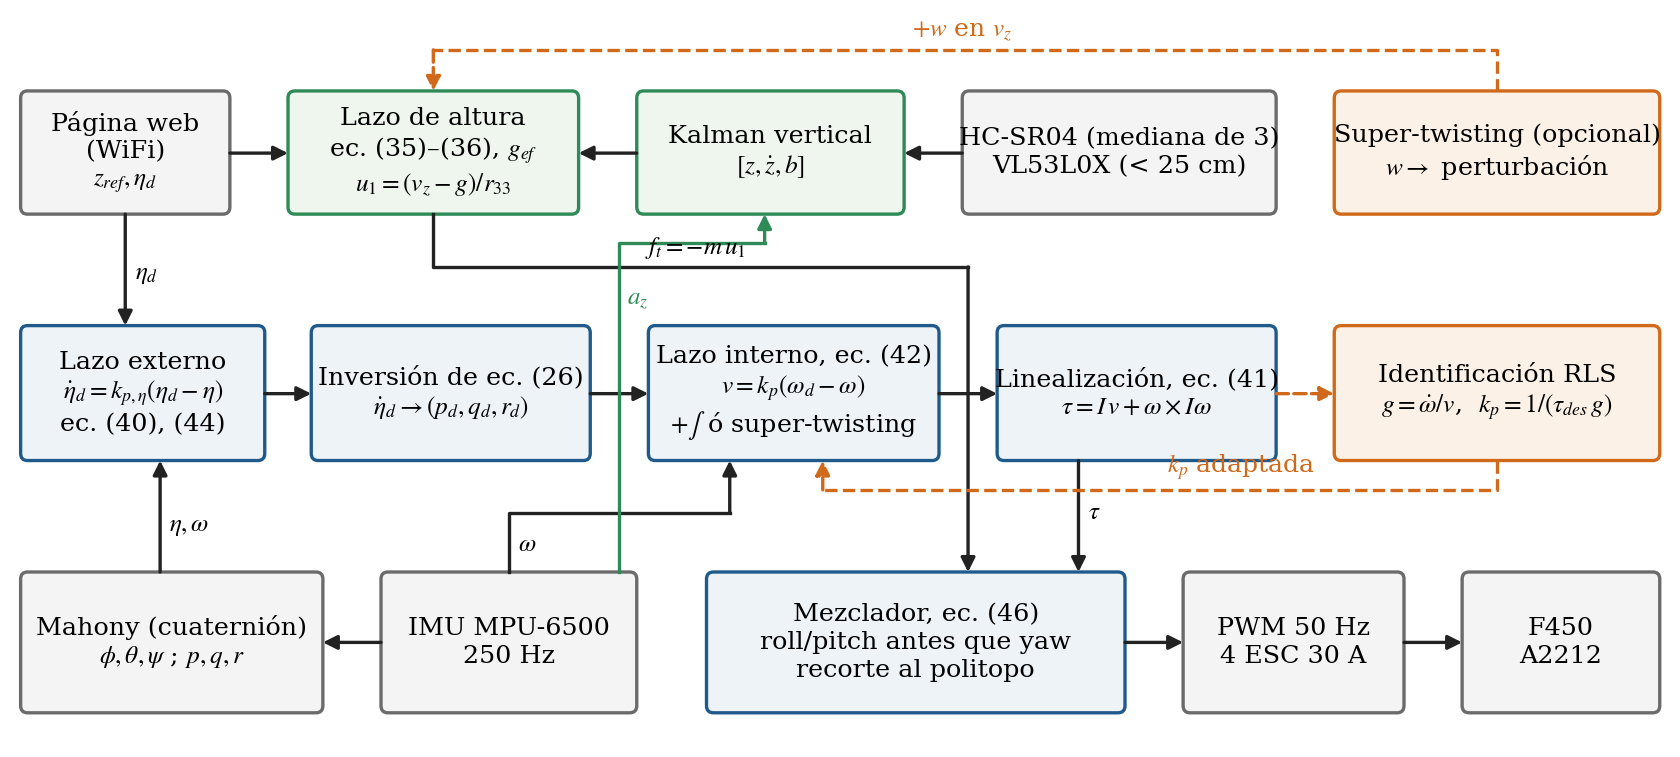
\includegraphics[width=0.93\textwidth]{f_arquitectura.png}
\caption{Arquitectura de control del firmware V\_11. En verde, el lazo de altura y su estimador; en azul, la cascada de actitud; en naranja, las extensiones robusta y adaptativa; en gris, sensores y actuadores.}
\label{fig:arq}
\end{figure*}

\textbf{Altura (ec. 35--36).} Con $v_z=\ddot z_d-k_{d,z}(\dot z-\dot z_d)-k_{p,z}(z-z_d)$ se impone $\ddot e_z+k_{d,z}\dot e_z+k_{p,z}e_z=0$ mediante
\begin{equation}
u_1=\frac{v_z-g_{ef}}{r_{33}},\qquad f_t=-m\,u_1,
\label{eq:altura}
\end{equation}
donde $g_{ef}$ es la prealimentación de hover: se carga al entrar en el modo MANTENER con el empuje que el dron está dando en ese instante ($g_{ef}=f_t r_{33}/m$, acotada a $[0.55,1.35]\,g$), en lugar de $g$ del modelo. Se añade un integrador ($k_{i,z}=1$, tope 2\,m/s$^2$, con anti-windup) y el empuje se acota a $[0.45,1.35]$ veces el de hover. Con $k_{p,z}=4$ y $k_{d,z}=3.6$ se tiene $\omega_n=2$\,rad/s y $\zeta=0.9$.

\textbf{Actitud.} El lazo externo impone $\dot\phi_d=k_{p,\phi}(\phi_d-\phi)$ (ec. 40; igual para $\theta$ y, con ec. 44, para $\psi$) y las velocidades deseadas del cuerpo salen de invertir (\ref{eq:euler}):
\begin{align}
p_d&=\dot\phi_d-\dot\psi_d\sin\theta,\nonumber\\
q_d&=\dot\theta_d\cos\phi+\dot\psi_d\cos\theta\sin\phi,\label{eq:inv}\\
r_d&=-\dot\theta_d\sin\phi+\dot\psi_d\cos\theta\cos\phi.\nonumber
\end{align}
El lazo interno es $v_p=k_{p,p}(p_d-p)$ (ec. 42, igual para $q$ y $r$) y el torque sale de la linealización (ec. 41)
\begin{align}
u_x&=I_xv_p+(I_z-I_y)qr,\nonumber\\
u_y&=I_yv_q+(I_x-I_z)pr,\label{eq:lin}\\
u_z&=I_zv_r+(I_y-I_x)pq.\nonumber
\end{align}
La Tabla~\ref{tab:gan} lista las ganancias por defecto. Con $k_{p,p}=15$\,s$^{-1}$ el lazo interno tiene constante de tiempo de $67$\,ms y con $k_{p,\phi}=6$\,s$^{-1}$ el externo, $167$\,ms, es decir, 2.5 veces más lento, como exige una cascada. El integrador de velocidad angular ($k_i$) viene en cero: primero se sintoniza el proporcional puro de las notas.

\begin{table}[t]
\caption{Ganancias y límites por defecto (\texttt{config.h}).}
\label{tab:gan}
\centering\small
\begin{tabular}{@{}lcc@{}}
\toprule
Lazo & Roll / Pitch & Yaw \\
\midrule
Ángulo $k_{p,\eta}$ [s$^{-1}$] & 6.0 & 2.5 \\
Velocidad angular $k_{p,\omega}$ [s$^{-1}$] & 15 & 5 \\
Super-twisting $(k_1,k_2)$ [rotación] & (3, 8) & (2, 5) \\
Altura $(k_{p,z},k_{d,z},k_{i,z})$ & \multicolumn{2}{c}{(4, 3.6, 1)} \\
Super-twisting altura $(k_1,k_2)$ & \multicolumn{2}{c}{(1.5, 2)} \\
Referencia máx. / corte de seguridad & \multicolumn{2}{c}{$25^\circ$ / $60^\circ$} \\
\bottomrule
\end{tabular}
\end{table}

\textbf{Mezclador con prioridad de ejes.} La inversa de (\ref{eq:mezcla}) da $\omega_i^2$. Como $k_fl/k_m=10.2$, un N\,m de yaw cuesta diez veces más rango de motor que uno de roll. Una caja negra previa mostró que el 94\,\% del rango de motor se gastaba en yaw y que el mezclador estaba saturado el 93\,\% del tiempo. Por ello V\_9 reparte por prioridad: primero el empuje, luego roll y pitch con todo el rango que necesiten (factor $s_{rp}\in[0,1]$) y el yaw con lo que sobre, nunca más del 30\,\% del recorrido. Sustituye al recorte componente a componente de las notas, que cambia la dirección del torque.

\textbf{Extensión robusta (super-twisting).} Tras la linealización cada lazo es $\dot s=v+d(t)$ con $d$ la incertidumbre del modelo. Con la superficie $s$ (error de velocidad angular, o $\sigma=\lambda(z_d-z)-\dot z$ en altura) se añade
\begin{equation}
v=k_1|s|^{1/2}\mathrm{sat}(s/\varphi)+w,\qquad \dot w=k_2\,\mathrm{sat}(s/\varphi),
\label{eq:st}
\end{equation}
que es el algoritmo de Levant~\cite{levant}, continuo, converge en tiempo finito si $k_2>L$ y $k_1>1.5\sqrt L$ con $|\dot d|\le L$, y cuyo estado $w$ estima $-d$. Se usa una capa límite $\varphi$ (0.10\,rad/s) para evitar el \emph{chattering} con el giroscopio ruidoso y el integrador se anula mientras está activo. Es la contraparte, en este dron, del SMC del bloque de control robusto del curso~\cite{notas2}.

\textbf{Extensión adaptativa (identificación recursiva).} Tras (\ref{eq:lin}) cada eje cumple $\dot\omega=g\,v$ con $g=1$ si el modelo es exacto. Se estima $g$ por mínimos cuadrados recursivos con olvido $\lambda=0.999$, aplicando el \emph{mismo} filtro de 8\,Hz a $\dot\omega$ y a $v$ (para que el desfase se cancele) y aprendiendo solo con excitación suficiente y sin saturación. Con $g$ se fija el ancho de banda y no la ganancia: $k_p=1/(\tau_{des}\,\hat g)$. Un $\hat g<0$ diagnostica un signo invertido.

\subsection{Estimación de estado}
\textbf{Actitud.} Filtro de Mahony~\cite{mahony} sobre cuaternión ($K_p=2$, $K_i=0.05$); la corrección solo se aplica si $0.5<|\bm a|<1.6$\,g. Sin magnetómetro el yaw deriva.

\textbf{Altura.} Filtro de Kalman~\cite{kalman} de tres estados $\bm x=[z,\dot z,b]^\top$ (z positivo hacia abajo, $b$ sesgo del acelerómetro). La predicción usa la aceleración vertical inercial $a_v=r_{31}a_x+r_{32}a_y+r_{33}a_z+g$ como entrada, y la corrección usa la distancia al suelo corregida por $r_{33}$. Manda el ultrasonido (mediana de 3 ecos), y el ToF solo bajo 25\,cm, con histéresis de 5\,cm en la frontera. La V\_11 re-sintoniza el filtro con el ruido medido en vuelo: $\sigma_{US}=0.05+0.08\,d$ (m), puerta de innovación de $4\sigma$, reanclaje tras 3 rechazos seguidos, $a_v$ filtrada a 20\,Hz y acotada a $\pm6$\,m/s$^2$, ruido de proceso mínimo de 3\,(m/s$^2$)$^2$ y deriva del sesgo $0.2$\,(m/s$^2$)$^2$/s. La medida de distancia se acepta solo entre 8\,cm y 3.5\,m (ultrasonido).

\subsection{Implementación, seguridad y desarrollo iterativo}
El lazo de control corre a 250\,Hz en el núcleo 1; los sensores a 20\,Hz y el servidor web en el núcleo 0. El PWM es de 50\,Hz, lo que impone un retardo de actuación de hasta 20\,ms y limita la ganancia útil del lazo interno. El arranque exige empuje 0 y dron casi nivelado; hay desarme a $60^\circ$ o si la IMU calla 100\,ms, y bajada automática si el enlace calla 0.8\,s.

El firmware se refinó en ciclos de vuelo--análisis--corrección (Tabla~\ref{tab:vers}); cada cambio responde a un hallazgo de una caja negra.

\begin{table}[t]
\caption{Evolución del firmware y su motivo.}
\label{tab:vers}
\centering\small
\begin{tabular}{@{}lp{6.1cm}@{}}
\toprule
Versión & Cambio y motivo \\
\midrule
V\_8 & Referencia de altura fija, nivel fino, página reducida. \\
V\_9 & Prioridad roll/pitch sobre yaw en el mezclador (94\,\% del rango en yaw). \\
V\_10 & Filtro del acelerómetro, solo medidas nuevas y crudas, rechazo de rebotes, hover aprendido; V\_10b: reanclaje del filtro porque la altura estimada divergía. \\
V\_11 & Kalman con el ruido medido del ultrasonido (13\,cm a 1.2\,m, no 4\,cm), mediana de ecos, $a_z$ filtrada y acotada, CSV sin duplicados. \\
\bottomrule
\end{tabular}
\end{table}

\subsection{Protocolo experimental y procesamiento}
La caja negra graba a 50\,Hz al armar y se descarga en CSV de 25 columnas: tiempo, modo, estado del mezclador, ángulos, velocidades angulares, altura estimada y de referencia, velocidad vertical, empuje, ambos sensores de distancia, mando por motor y aceleración vertical. Todos los vuelos son del 26-nov-2026. Se analizan los registros recortados a los tramos de interés (los huecos se detectan por saltos de tiempo $>0.1$\,s y no se unen): dos vuelos V\_11 (A: 19:09:36, 21.0\,s; B: 19:25:45, 33.0\,s) y cinco de V\_10/V\_10b como referencia. Las métricas se calculan sobre las muestras con altura estimada $>0.15$\,m (``en el aire''), con el script \texttt{make\_figures.py}. Las ganancias son las por defecto de la Tabla~\ref{tab:gan}. El CSV no registra la referencia de actitud ni los interruptores robusto/adaptativo, que por defecto están apagados, ni la tensión de batería.

\section{Resultados}
\label{sec:res}

\subsection{Parámetros identificados}
La Tabla~\ref{tab:par} reúne los parámetros y la Fig.~\ref{fig:ident} los datos de los ensayos. Las inercias cumplen $I_x<I_y<I_z$ con incertidumbres estándar combinadas de $1.4$, $1.6$ y $2.2$\,\% (Anexo~A); $I_z$ es la más dispersa porque sus cinco períodos van de 4.28 a 4.54\,s. Además $I_x+I_y$ difiere de $I_z$ en un $0.9$\,\%, compatible con cero, como se espera de un cuerpo casi plano. Con ellas, la autoridad de roll en hover es de $0.34$\,N\,m, equivalente a unos $35$\,rad/s$^2$ ($\approx2000^\circ$/s$^2$), calculada con los parámetros del firmware. Con $\omega_{\max}=1046$\,rad/s el empuje máximo es $14.05$\,N (relación empuje/peso $1.43$) y el hover cae en el $70$\,\% del acelerador. Con $k_fl/k_m=10.2$, el yaw es diez veces más caro que el roll en rango de motor.

\begin{table}[t]
\caption{Parámetros del dron. Incertidumbre estándar combinada (Anexo~A).}
\label{tab:par}
\centering\footnotesize\setlength{\tabcolsep}{3pt}
\begin{tabular}{@{}lll@{}}
\toprule
Parámetro & Valor & Unidad \\
\midrule
Masa $m$ & 1.0022 & kg \\
Brazo efectivo $l$ & 0.1616 & m \\
$I_x$ & $(9.71\pm0.13)\times10^{-3}$ & kg\,m$^2$ \\
$I_y$ & $(10.56\pm0.17)\times10^{-3}$ & kg\,m$^2$ \\
$I_z$ & $(20.08\pm0.45)\times10^{-3}$ & kg\,m$^2$ \\
$K_f$ (hoja, 1000--1500\,\textmu{}s) & $3.91\times10^{-6}$ & N/\textmu{}s$^2$ \\
$a$ (ajuste cuadrático, 13 pts) & $(3.42\pm0.34)\times10^{-6}$ & N/\textmu{}s$^2$ \\
$K_m=\alpha^2K_f$ (hoja) & $6.19\times10^{-8}$ & N\,m/\textmu{}s$^2$ \\
$K_m=\alpha^2a$ (ajuste, Anexo~A) & $(5.42\pm0.53)\times10^{-8}$ & N\,m/\textmu{}s$^2$ \\
$k_f$ (firmware) & $3.2107\times10^{-6}$ & N/(rad/s)$^2$ \\
$k_m$ (firmware) & $5.088\times10^{-8}$ & N\,m/(rad/s)$^2$ \\
\bottomrule
\end{tabular}
\end{table}

\begin{figure*}[t]
\centering
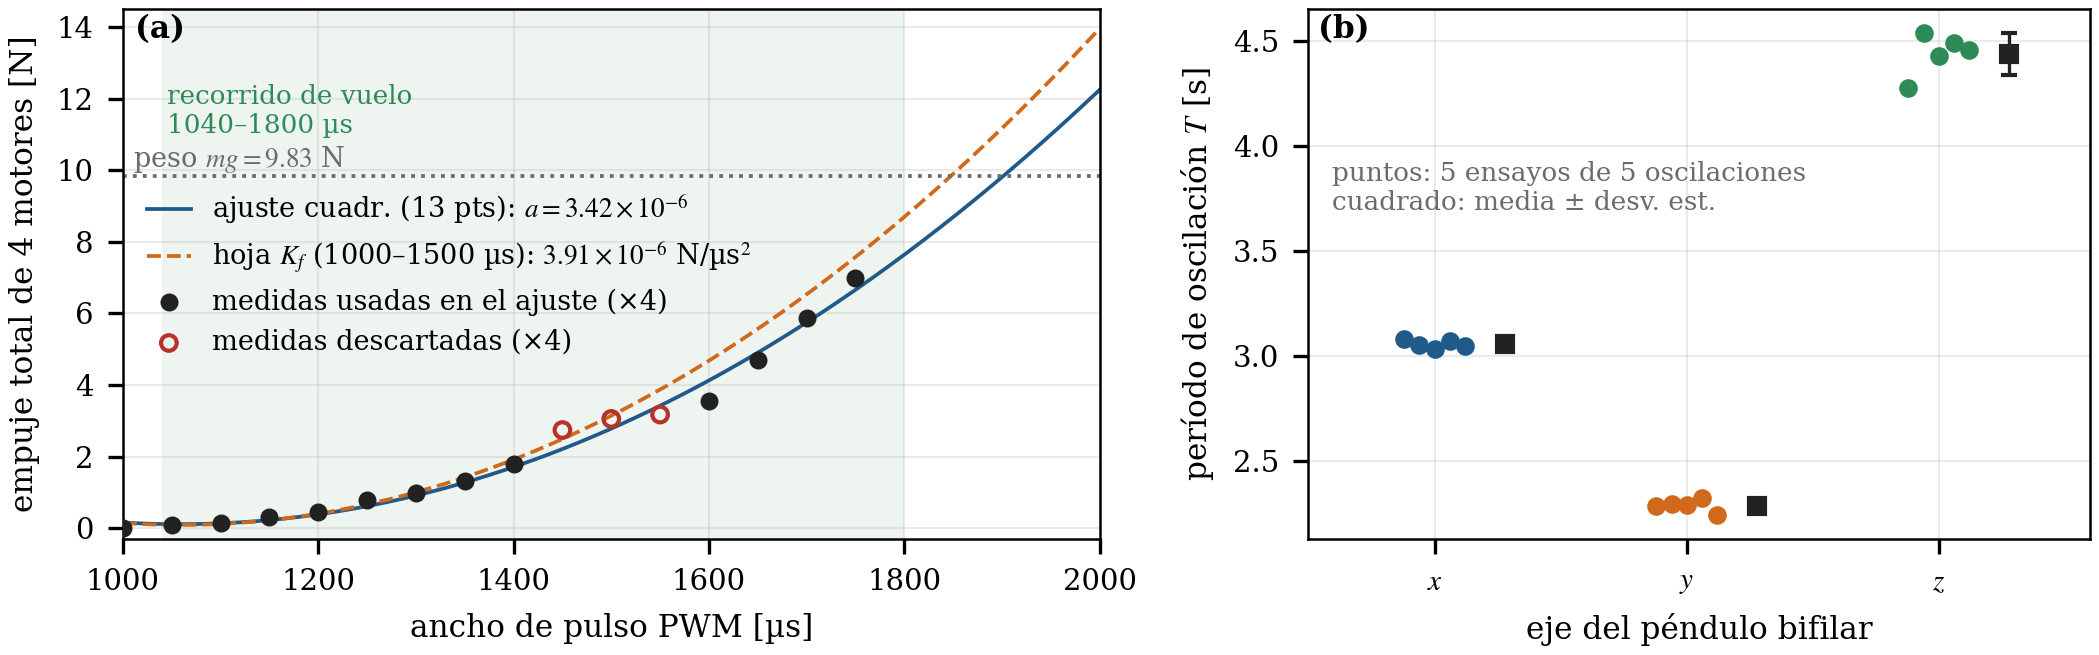
\includegraphics[width=0.93\textwidth]{f_ident.png}
\caption{Ensayos de identificación. (a) Empuje total (cuatro motores) frente al pulso PWM, con el ajuste cuadrático y la curva de la hoja. (b) Períodos medidos en el péndulo bifilar.}
\label{fig:ident}
\end{figure*}

El coeficiente $K_f$ depende del rango de ajuste: la hoja da $3.91\times10^{-6}$ usando los puntos de 1000 a 1500\,\textmu{}s y el ajuste cuadrático de los 13 puntos filtrados da $3.42\times10^{-6}$, un $12.5$\,\% menos ($R^2=0.987$ y $0.992$). La diferencia crece al extrapolar: a 2000\,\textmu{}s predicen $13.8$ y $12.2$\,N en total. Más importante, la curva de banco no es transferible al vuelo. En el vuelo B los cuatro motores trabajaron en promedio al $87$\,\% del recorrido, unos $1700$\,\textmu{}s, donde la curva de banco da $5.7$--$6.4$\,N en total, menos que el peso ($9.83$\,N), y sin embargo el dron voló. Las causas posibles son la recalibración de los ESC a 1040--1800\,\textmu{}s, la tensión de batería durante el ensayo y la medición con balanza; los datos no permiten separarlas. El firmware evita el problema suponiendo $\omega$ lineal en el recorrido calibrado y tratando $\omega_{\max}$ como parámetro de ajuste.

\subsection{Vuelos con V\_11: actitud}
La Fig.~\ref{fig:vueloB} muestra el vuelo B y la Tabla~\ref{tab:vuelos} resume los dos vuelos. En B el empuje se aplicó en $t=0.9$\,s, el dron superó 0.3\,m en $3.3$\,s y alcanzó $1.48$\,m en $5.6$\,s. Después descendió lentamente desde $\approx0.6$\,m ($t\approx8$\,s) hasta tocar el suelo en $t\approx19.4$\,s.

\begin{figure}[t]
\centering
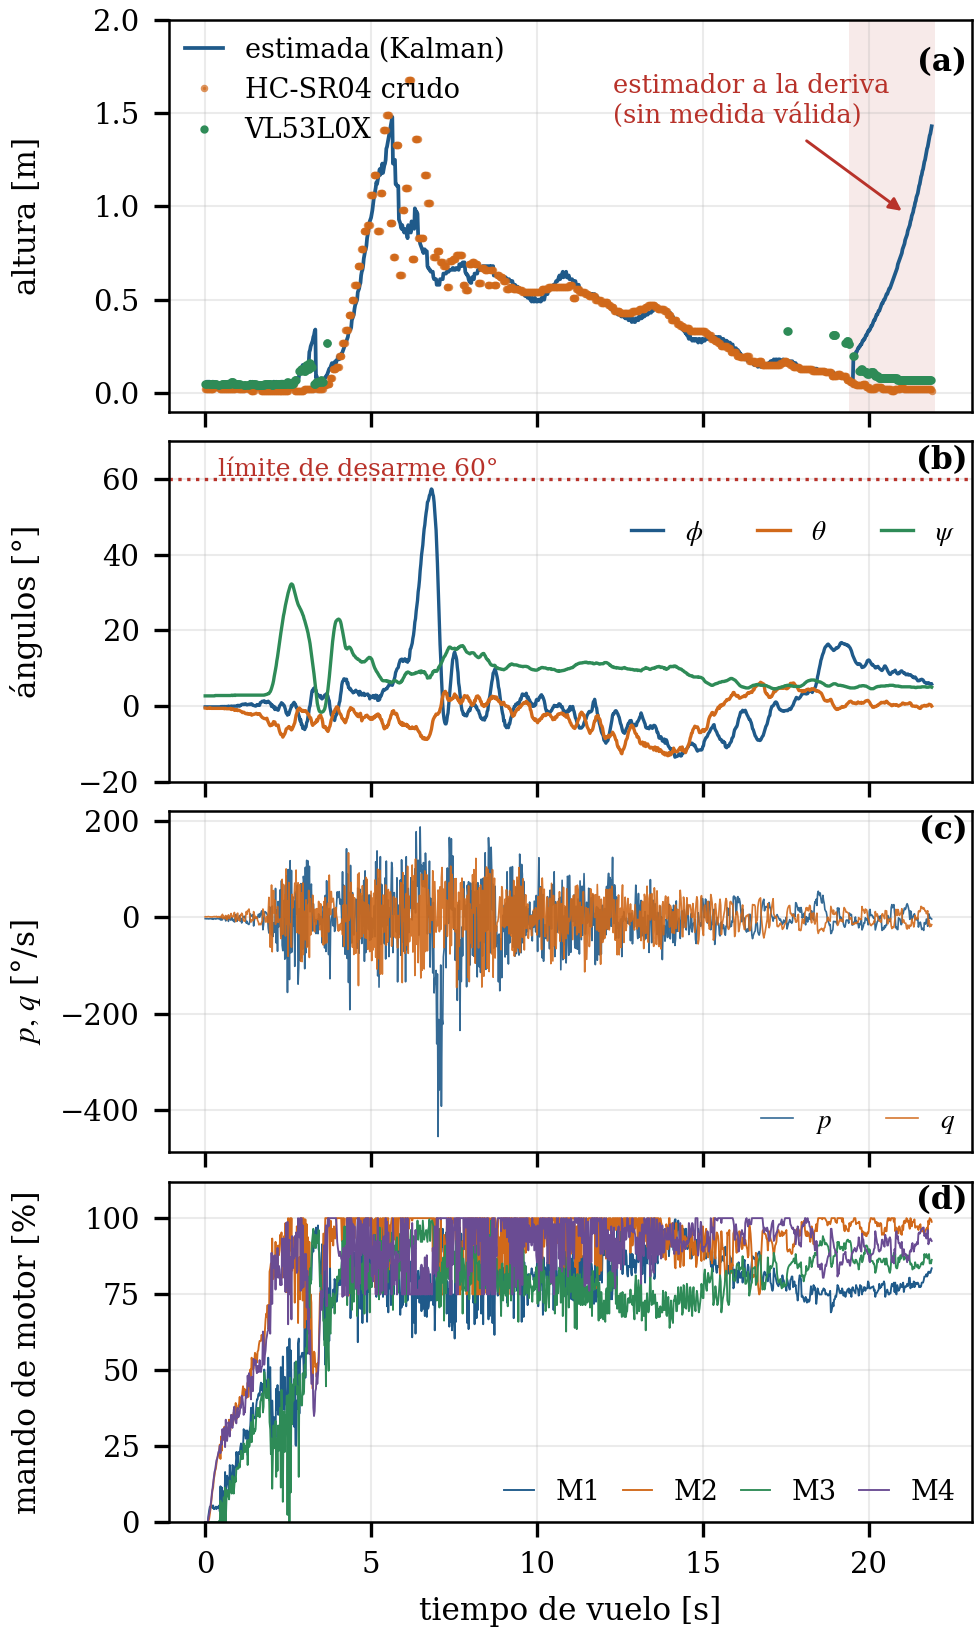
\includegraphics[width=0.97\linewidth]{f_vuelo_B.png}
\caption{Vuelo B (V\_11): (a) altura estimada y sensores; (b) ángulos de Euler; (c) velocidades angulares $p$ y $q$; (d) mando de cada motor. La banda roja marca el tramo sin medida válida tras la toma de contacto.}
\label{fig:vueloB}
\end{figure}

\begin{table}[t]
\caption{Métricas de los vuelos V\_11 (muestras con altura $>0.15$\,m).}
\label{tab:vuelos}
\centering\footnotesize\setlength{\tabcolsep}{3pt}
\begin{tabular}{@{}lcc@{}}
\toprule
Métrica & A & B \\
\midrule
Duración registrada [s] & 21.0 & 33.0 \\
Muestras en el aire & 578 & 808 \\
Altura estimada máxima [m] & 1.77 & 1.48 \\
Roll: media / desv. / máx. [$^\circ$] & 8.9 / 5.4 / 18.9 & 2.2 / 11.5 / 57.4 \\
Pitch: media / desv. / máx. [$^\circ$] & $-7.5$ / 3.1 / 15.8 & $-2.6$ / 4.5 / 13.1 \\
Tiempo con $|\phi|<10^\circ$ [\%] & 51 & 78 \\
$\sigma_p,\sigma_q,\sigma_r$ [$^\circ$/s] & 49 / 45 / 14 & 62 / 44 / 14 \\
Mezclador saturado [\%] & 11 & 16 \\
Motor 2 / motor 4 al $\ge99$\,\% [\%] & 43 / 0 & 37 / 25 \\
Empuje pedido medio [N] & 9.59 & 11.33 \\
\bottomrule
\end{tabular}
\end{table}

La actitud se mantuvo acotada en ambos vuelos, sin desarmes por inclinación. En B, el $90$\,\% del tiempo estuvo con $|\theta|<10^\circ$ y el $78$\,\% con $|\phi|<10^\circ$. Hay un evento relevante: un pico de roll de $57.4^\circ$ en $t=6.8$\,s (con $|p|$ hasta unos $450^\circ$/s), a $2.6^\circ$ del umbral de desarme de $60^\circ$, que se recuperó en menos de un segundo (el roll estuvo $0.62$\,s por encima de $30^\circ$). El yaw se mantuvo entre $-1.6^\circ$ y $32^\circ$ y presenta dos excursiones al despegar, de $32^\circ$ y $23^\circ$. En A el roll y el pitch tienen medias de $+8.9^\circ$ y $-7.5^\circ$; como el CSV no guarda la referencia de actitud, no se puede separar si es error de seguimiento, un nivel (trim) mal ajustado o una orden del piloto.

El contenido espectral (vuelo B, $t=4.5$--$21.9$\,s) muestra que la oscilación no es de baja frecuencia: el $82$--$90$\,\% de la varianza de $\phi$ y $\theta$ está bajo 1\,Hz, pero el $82$\,\% de la de $q$ está entre 8 y 25\,Hz. Las desviaciones de 44--62$^\circ$/s en $p$ y $q$ (Fig.~\ref{fig:vueloB}c) serían entonces sobre todo ruido y vibración del giroscopio realimentados al mezclador, lo que se refleja en un mando de motor muy movido (Fig.~\ref{fig:vueloB}d). Es una interpretación: la caja negra muestrea a 50\,Hz, de modo que el contenido por encima de 25\,Hz se pliega sobre la banda observada, y no hay un registro a 250\,Hz con el que confirmarlo.

\subsection{Actuación y saturación}
El mezclador estuvo saturado el 11\,\% (A) y el 16\,\% (B) de las muestras en el aire, y el motor 2 trabajó al $\ge99$\,\% del recorrido el 43 y el 37\,\% del tiempo (el motor 4 el 25\,\% en B). La prioridad de V\_9 protege roll y pitch frente al yaw, pero no crea margen: el hover exige $\approx70$\,\% del acelerador y el empuje pedido medio fue de 9.6 y 11.3\,N ($68$ y $80$\,\%), de modo que en B queda poca reserva para corregir. En la fase de descenso lento de B ($t=8$--$19.4$\,s, altura $0.59\to0.06$\,m, $\bar{\dot z}=-0.05$\,m/s) el empuje pedido fue constante a $11.4$\,N, un $16$\,\% sobre $mg$; en el vuelo A, en un tramo de descenso lento ($t=13$--$16.7$\,s, altura $0.79\to0.45$\,m, $\bar{\dot z}=-0.03$\,m/s) fue de $7.8$\,N, un $21$\,\% bajo $mg$. El empuje de hover \emph{pedido} cambió un $46$\,\% entre dos vuelos del mismo día. Como el dron no mide la tensión de batería, el registro no permite atribuirlo a su descarga.

\subsection{Altura: lazo cerrado y estimador}
La Fig.~\ref{fig:holdA} muestra el único tramo en MANTENER ALTURA de los dos vuelos V\_11 (A, $t=0.78$--$3.38$\,s, 120 muestras). El modo se activó con el dron subiendo a $\approx0.65$\,m/s y $11.0$\,N, de modo que la ec. (\ref{eq:altura}) aprendió $g_{ef}\approx11$\,m/s$^2$ ($\approx1.1\,g$) como si fuera el hover. La altura estimada superó la referencia (0.36\,m y luego 0.96\,m) hasta 1.16\,m, y el error cuadrático medio en el tramo es de $0.24$\,m (máximo $0.60$\,m). Con un solo tramo de 2.6\,s no se puede afirmar que el lazo de altura cumpla su diseño ($\omega_n=2$\,rad/s). La prealimentación aprendida solo es válida si el modo se activa cerca del hover.

\begin{figure}[t]
\centering
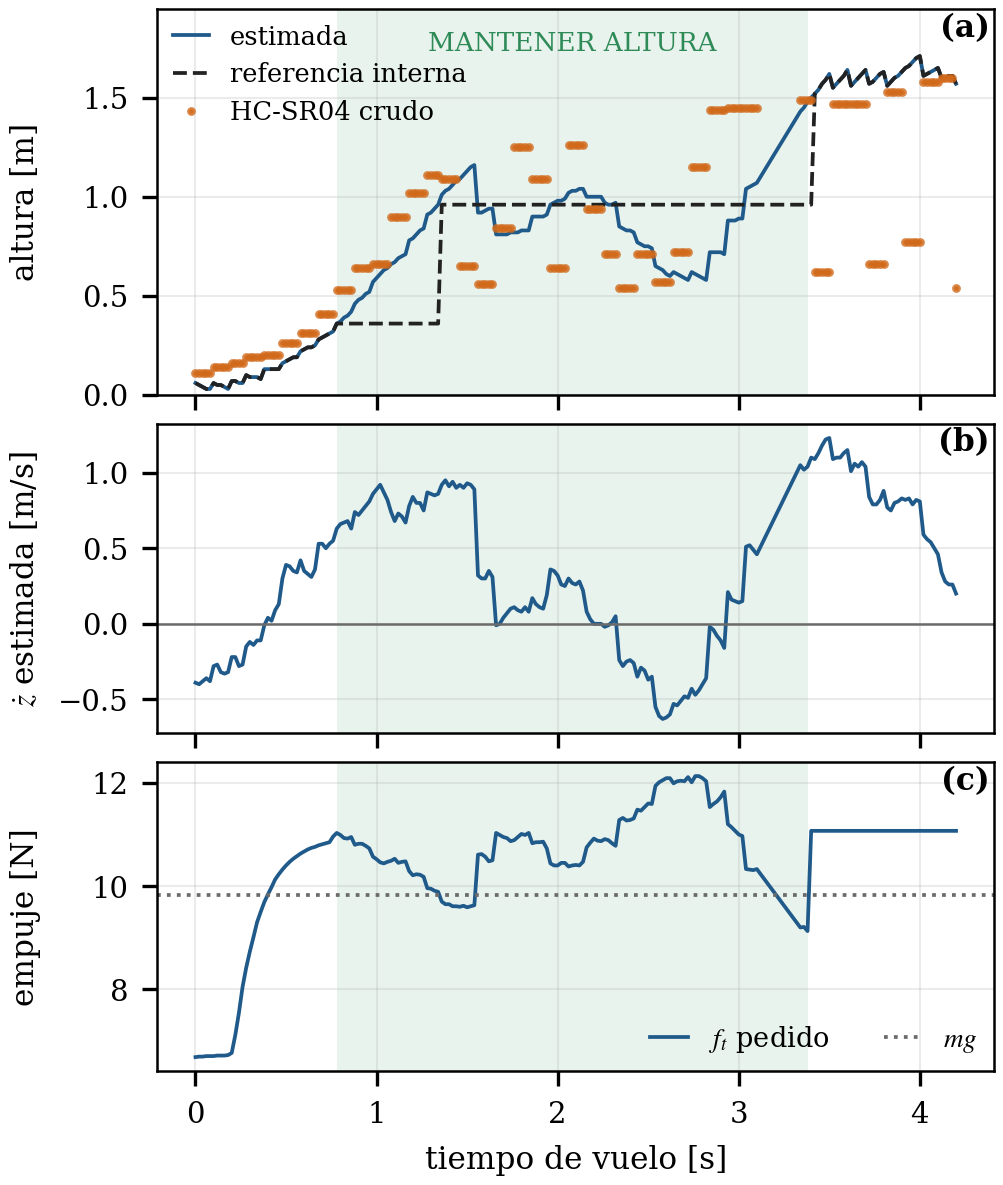
\includegraphics[width=0.93\linewidth]{f_hold_A.png}
\caption{Vuelo A (V\_11), modo MANTENER ALTURA (banda verde): (a) altura, (b) velocidad vertical estimada, (c) empuje pedido.}
\label{fig:holdA}
\end{figure}

La Tabla~\ref{tab:est} compara el estimador de altura entre versiones usando como indicador la diferencia con la lectura del ultrasonido y la fracción de muestras con altura estimada negativa, físicamente imposible. En el vuelo V\_10 de las 16:50 la altura estimada oscila con amplitud de varios metros alrededor de lecturas de ultrasonido de $0.3$--$1$\,m (Fig.~\ref{fig:estimador}a) y el $35$\,\% de las muestras tiene altura negativa; los otros cuatro vuelos de V\_10/V\_10b son mejores ($0.26$--$0.58$\,m). En V\_11-B la desviación es de $0.12$\,m y solo el $1$\,\% de las muestras difiere más de $0.5$\,m. Por encima de $0.8$\,m el ultrasonido crudo se aparta mucho de la altura estimada ($\approx0.3$--$0.4$\,m, frente a los $0.13$--$0.18$\,m del modelo $\sigma_{US}$); la puerta de innovación hace el resto.

\begin{table}[t]
\caption{Estimador de altura frente a la lectura del ultrasonido.}
\label{tab:est}
\centering\small
\begin{tabular}{@{}lccc@{}}
\toprule
Vuelo & Desv. [m] & $|\mathrm{res}|>0.5$\,m [\%] & Alt.\,$<0$ [\%] \\
\midrule
V\_10, 16:50 & 1.39 & 36.8 & 34.7 \\
V\_10, 17:42 & 0.31 & 7.6 & 2.3 \\
V\_10, 17:45 & 0.26 & 3.2 & 0.0 \\
V\_10b, 18:32 & 0.39 & 4.5 & 0.6 \\
V\_10b, 18:36 & 0.58 & 23.6 & 2.1 \\
V\_11, A (19:09) & 0.30 & 11.8 & 8.3 \\
V\_11, B (19:25) & 0.12 & 1.0 & 0.0 \\
\bottomrule
\end{tabular}
\end{table}

\begin{figure}[t]
\centering
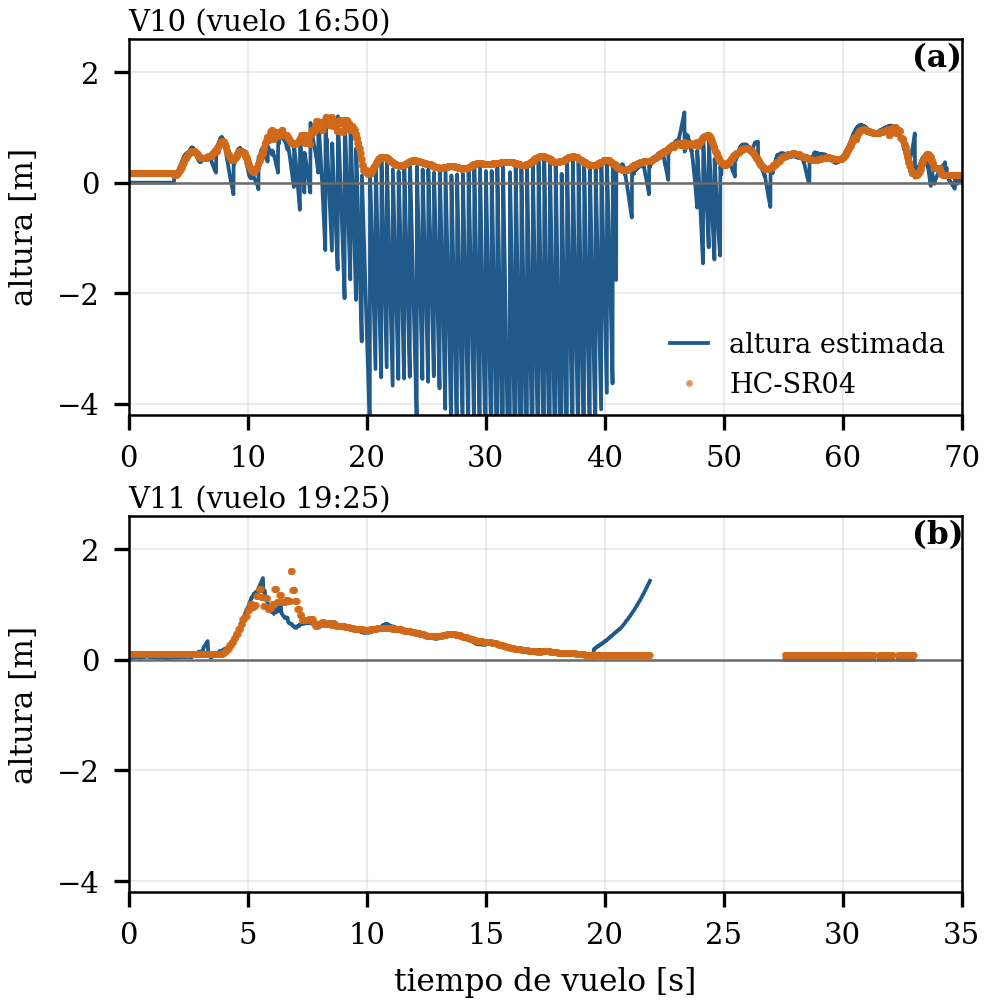
\includegraphics[width=0.93\linewidth]{f_estimador.png}
\caption{Altura estimada y lectura del ultrasonido: (a) V\_10, con oscilaciones del estimador por debajo del suelo; (b) V\_11 (vuelo B).}
\label{fig:estimador}
\end{figure}

La mejora no es uniforme. En V\_11-A hay un $8$\,\% de muestras negativas y en ambos vuelos V\_11 el estimador falla al final. En B, tras tocar el suelo ($t=19.4$\,s) el ultrasonido crudo lee $0.02$--$0.05$\,m, bajo su mínimo válido de $0.08$\,m; el ToF registra $0.07$--$0.10$\,m, pero el log marca \texttt{alt\_ok}=0 desde $t=20.6$\,s. Con el empuje aún en $11.4$\,N, la estimación sube de $0.06$ a $1.34$\,m en 2.4\,s, como si integrara la aceleración sin ancla (Fig.~\ref{fig:vueloB}a). En A ocurre lo contrario: tras $t=19.6$\,s (\texttt{alt\_ok}=0, con el ToF leyendo $0.05$--$0.06$\,m) la altura estimada cae hasta $-1.0$\,m. Las columnas registradas no permiten explicar por qué el ToF no ancla el filtro. Con dos vuelos V\_11 la comparación con V\_10 es indicativa, no concluyente.

\subsection{Discusión y limitaciones}
\label{sec:disc}
\emph{Qué funcionó.} La cascada de actitud del curso, con los parámetros identificados, bastó para despegar, subir a $1.5$\,m y volver al suelo sin desarme por inclinación en vuelos de 20--30\,s. El mezclador por prioridad y el Kalman re-sintonizado atienden los dos problemas que mostraron los registros de V\_9 y V\_10, el segundo con mejora parcial.

\emph{Qué no está demostrado.} (i) El lazo de altura cerrado solo tiene 2.6\,s de datos y con un error rms de $0.24$\,m. (ii) Las extensiones del curso (super-twisting y adaptación RLS) están implementadas y se describen, pero el CSV no registra su estado ni $\hat g$ ni $w$, y por defecto están apagadas: no hay evidencia de vuelo de que mejoren el resultado. (iii) El estimador diverge cuando el log marca \texttt{alt\_ok}=0 junto al suelo.

\emph{Limitaciones del modelo y de la instrumentación.} Hay una brecha de $K_f$ y empuje entre banco y vuelo; el empuje de hover pedido varió un $46$\,\% entre vuelos; no hay medición de batería ni de posición lateral; sin magnetómetro el yaw deriva; y el PWM a 50\,Hz limita el ancho de banda del lazo interno. La consecuencia práctica es poca reserva de empuje: el motor 2 trabaja al $\ge99$\,\% del recorrido entre el 37 y el 43\,\% del tiempo.

\section{Conclusiones}
\label{sec:conc}

\begin{itemize}
\item Se implementó en un ESP32-S3 a 250\,Hz la cascada de control del curso (ángulo $\to$ velocidad angular $\to$ torque, altura con cancelación de gravedad y mezclador por inversión) con parámetros identificados: $I_x=9.71$, $I_y=10.56$, $I_z=20.08\times10^{-3}$\,kg\,m$^2$ con incertidumbres combinadas de $1.4$--$2.2$\,\% (Anexo~A), el coeficiente de empuje de banco y el de par a partir de la relación empuje/par de la hélice.
\item En dos vuelos V\_11 no hubo desarme por inclinación; en B el dron despegó, llegó a 1.5\,m y volvió al suelo, con $|\phi|<10^\circ$ el $78$\,\% del tiempo y un pico de $57^\circ$ recuperado en menos de un segundo. La actitud queda acotada pero ruidosa: el $82$\,\% de la varianza de $q$ está entre 8 y 25\,Hz.
\item El Kalman de altura con el ruido medido del ultrasonido redujo la desviación frente al sensor de $0.26$--$1.39$\,m (V\_10) a $0.12$\,m (V\_11-B), pero diverge junto al suelo cuando el log marca \texttt{alt\_ok}=0 (B: de $0.06$ a $1.34$\,m; A: hasta $-1.0$\,m); falta una política explícita para ese caso.
\item La brecha entre modelo y vuelo es el principal límite: la curva de empuje de banco no explica el vuelo, el empuje de hover pedido varió un $46$\,\% entre vuelos, y la relación empuje/peso de $1.43$ deja el motor 2 al $\ge99$\,\% del recorrido entre el 37 y el 43\,\% del tiempo.
\item El lazo de altura cerrado solo se observó 2.6\,s (error rms $0.24$\,m) y las extensiones robusta y adaptativa no se registraron en vuelo, por lo que no hay evidencia de su efecto.
\end{itemize}

\textbf{Trabajo futuro.} Registrar en el CSV la referencia de actitud, el estado del super-twisting y de la adaptación ($w$, $\hat g$) y la tensión de batería; repetir el ensayo de empuje con los ESC en su calibración final; añadir derivada o un filtro en el lazo de velocidad angular; activar MANTENER ALTURA solo cerca del hover y suspender el estimador si no hay medida válida bajo 8\,cm; y añadir un sensor de posición lateral.


\begin{thebibliography}{9}
\bibitem{notas1} O.~E. Ramos Ponce, \emph{Robots Aéreos}, notas de clase, Robótica Avanzada 2026-2, UTEC.
\bibitem{notas2} O.~E. Ramos Ponce, \emph{Control Adaptativo y Robusto en Robótica}, notas de clase, Robótica Avanzada 2026-2, UTEC.
\bibitem{mahony} R.~Mahony, T.~Hamel and J.-M. Pflimlin, ``Nonlinear complementary filters on the special orthogonal group,'' \emph{IEEE Trans. Autom. Control}, vol.~53, no.~5, pp.~1203--1218, 2008.
\bibitem{kalman} R.~E. Kalman, ``A new approach to linear filtering and prediction problems,'' \emph{J. Basic Eng.}, vol.~82, no.~1, pp.~35--45, 1960.
\bibitem{levant} A.~Levant, ``Sliding order and sliding accuracy in sliding mode control,'' \emph{Int. J. Control}, vol.~58, no.~6, pp.~1247--1263, 1993.
\bibitem{jardin} M.~R. Jardin and E.~R. Mueller, ``Optimized measurements of unmanned-air-vehicle mass moment of inertia with a bifilar pendulum,'' \emph{J. Aircraft}, vol.~46, no.~3, pp.~763--775, 2009.
\end{thebibliography}
\end{document}
